\chapter{ソフトウェアによる実験}
\label{chap:software-experimentation}

ソフトウェアによる実装では、汎用的なPCに10Gbpsに対応したNIC、4K対応キャプチャボード Blackmagic Design Intensity Pro 4Kを用いて行った。
本実装の概要を、図\ref{fig:software-implement-flow}に示す。

\begin{table}[htbp]
  \caption{ソフトウェアによる実装を検証したPCの構成}
  \label{tb:software-specification}
  \begin{center}
  \begin{tabular}{c||c}
    \hline
    OS  & Ubuntu 14.04 Desktop \\\hline
    CPU & Intel Core i7-4770 @ 3.40GHz \\\hline
    RAM & 8GB                  \\\hline
  \end{tabular}\end{center}
\end{table}

\begin{figure}[htbp]
    \begin{center}
        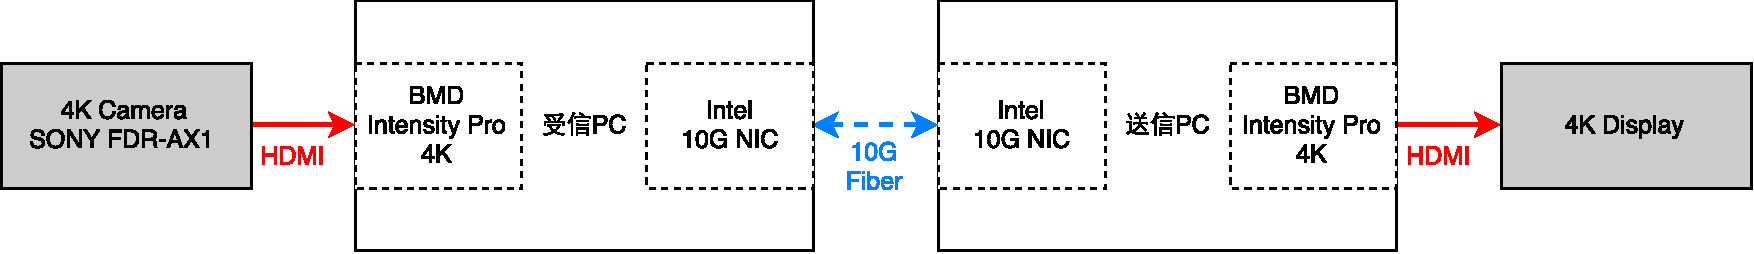
\includegraphics[bb=0 0 841 121,width=15.5cm]{img/software-implement-flow.pdf}
    \end{center}
    \caption{ソフトウェアによる実装の構成}
    \label{fig:software-implement-flow}
\end{figure}

\begin{figure}[htbp]
    \begin{center}
        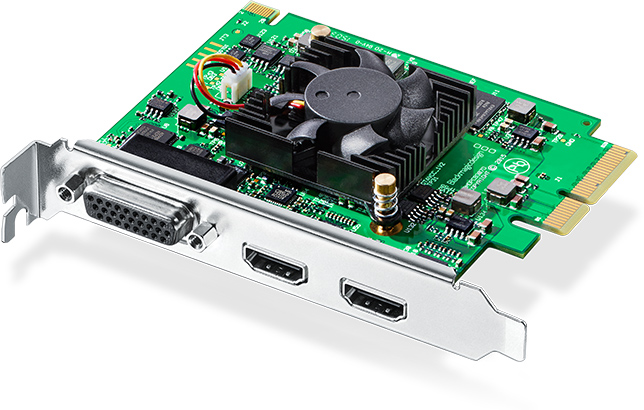
\includegraphics[bb=0 0 644 410,width=5cm]{img/bmd-intensity-pro-4k.jpg}
    \end{center}
    \caption{Blackmagic Design Intensity Pro 4K キャプチャーボード}
    \label{fig:ted-4k-fmc-card}
\end{figure}

送信プログラムでは、キャプチャボードでキャプチャしたデータをBlackmagic DeckLink SDK\cite{bmd-decklink-sdk}を用いて取得し、IP経由で伝送するプログラムを作成した。
受信プログラムでは、IP経由で受信したデータをLinux汎用的なメディアプレーヤーであるmplayerで再生するプログラムを作成した\cite{bmd-4k-streaming}。
% ここは後ほど詳細を記述する。

今回の評価ではダークファイバー環境での想定のため、順序制御、再送制御の実装を省くため、TCPで実装を行った。

% \begin{itembox}[l]{{\tt 03.tex}}
% \begin{verbatim}
% \begin{figure}[htbp]
%     \begin{center}
%        \fbox{\includegraphics[width=40mm,bb=0 0 640 480]{img/image.jpg}}
%     \end{center}
%     \caption{図の例}
%     \label{fig:sample1}
% \end{figure}
% \end{verbatim}
% \end{itembox}
